\documentclass[a4paper,11pt,report]{scrartcl}
\usepackage[dutch]{babel}
\usepackage[T1]{fontenc}
\usepackage[utf8]{inputenc}
\usepackage{lmodern}
\usepackage{amssymb}
\usepackage{color}
\usepackage{graphicx}
\usepackage{mathtools}
\DeclareGraphicsExtensions{.pdf,.png,.jpg}
\newcommand{\tab}{\hspace*{2em}}

\title{\huge\textbf{Deliverable 3}}
\author{Piet van Agtmaal 4321278\\
	    Jochem Heijltjes 1534041\\
		Arthur Hovanesyan 4322711\\
		Paul Bakker 4326091\\
		Jente Hidskes 4335732
	   }

\begin{document}
\begin{titlepage}
\maketitle
\thispagestyle{empty} %geen page numbering op opening pagina
\end{titlepage}

\newpage\section{Introduction}

2048 is a very popular game created by by Gabriele Cirulli, based on 1024 by
Veewo Studio and conceptually similar to Threes by Asher Vollmer.\\

We are five Computer Science students at the Delft University of Technology,
The Netherlands. We created a clone of the original 2048 game for the course
Software Engineering Methods.\\

We didn't just make a clone of the original 2048 game, we also added
multiplayer functionality. Now you can challenge your neighbours, your
coworkers, your kids or even the Queen of England to play a game of 2048!\\

This document tells you everything you need to know to get started. Technical aspects of
the game are covered in here as well.\\

Setting up a multiplayer game is really straightforward, however. Just make sure incoming connections to port TCP/2048 reach the hosting machine! Yes, port 2048! Who would have thunk* it? More details are up ahead!\\

Good luck and have fun!\\

\textbf{P.S.:} We, the developers, are not reliable in case of frustration. ;)\\

\textbf{*} See: http://english.stackexchange.com/questions/55577/proper-usage-of-the-word-thunk

\newpage\section{How to play 2048}

This section briefly describes how to play 2048 and provides information on
the functionality it has, such as playing the game alone, with friends and how
to use the logging features.\\

\subsection{Singleplayer game}
After starting the application you will see the main menu. In the main menu,
click the \texttt{Singleplayer} button to start your singleplayer game.\\

You move the tiles with the arrow keys. Each time two tiles with the same
number collide, the numbers are added and the two tiles merge. Your goal is to
reach the 2048 tile!\\

To return to the menu, press the \texttt{Escape} button any time. Don't worry,
your current game will be saved for you! (This also applies to closing the
game!).

\subsection{Multiplayer game}
The multiplayer version is identical to the singleplayer, except here you will
compete against a friend, colleague, coworker or your worst enemy over LAN or
the internet. Your opponent does not have to be in the same room with you; they
can even be on the other side of the planet and you can still kick their
asses!\\

Your goal is to reach the 2048 tile \textit{before} your opponent does. In case you
are unable to reach the 2048 tile (e.g., because you died), your opponent
automatically wins.\\

We will now briefly explain how to connect to eachother. Please refer to the
documentation of your networking equipment or software in case you experience
networking problems.

\subsubsection{Joining a game}
To connect to another player, choose the \texttt{Join a game} button in the
main menu. The application will try to connect to the remote address you
entered, on port 2048, using TCP.

\subsubsection{Hosting a game}
To have another player connect to you, choose the \texttt{Host a game} button
in the main menu. The application will bind to port 2048/TCP on all the
system's network interfaces. In case you wish to play over the internet,
please make sure connections on this port are forwarded to your local address
on your NAT device.

\subsection{Logging}
The game supports several commandline arguments for logging.\\

By default, the application will log to the standard output, using the
\texttt{INFO} logging level. If enabled, however, errors will be logged to
\texttt{stderr}. The logging level can also be adjusted.\\

The supported arguments are:
\begin{verbatim}
$ jarfile.jar [logLevel] [file]
\end{verbatim}
or, otherwise:
\begin{verbatim}
$ Launcher.java [logLevel] [file]
\end{verbatim}
Both of these fields are parsed case-insensitively.\\

Two examples:
\begin{verbatim}
$ Launcher.java debug
\end{verbatim}
will run the game and log all debug and info messages. 
\begin{verbatim}
$ Launcher.java error file
\end{verbatim}
will run the game and log all debug, error and info messages to the system's
output streams (\texttt{stdout} and \texttt{stderr}) and will write them to a
new file as well.\\

Please see the corresponding section below for more information on the possible
arguments:\\

\textbf{logLevel} can be one of the following:
\begin{description}
	\item[all] logs all messages;
	\item[info] logs info messages only;
	\item[error] log error messages and info messages;
	\item[debug] log debug, error and info messages;
	\item[none] disables logging.
\end{description}

\textbf{file}

Setting the \texttt{file} flag will write all messages of the previously set
logging level to a file. By default, a new file with the format
\texttt{2048\_YYYYMMDD\_HHmmss.log} will be created, where
\texttt{YYYMMMDDD\_HHmmss} is the time of application start.

\newpage\section{Test report}

In this section we will explain how we tested our game. We will start by
explaining how often we tested our game. Afterwards, we will explain what
kinds of testing we have done. Lastly, we will present the results of the
testing procedure.

\subsection{Test frequency}
In this section we will discuss how frequently we tested our game. Due to the
design patters we implemented, testing was essential. We tested using our
unit tests (locally and on Devhub as well) and visual tests. Implementing
iterators caused some problems that only arised during our visual tests. These
were, however, resolved immediately.

\subsection{Testing methods}
Visual tests involved actually playing the game and analyzing logging output
manually. Unit tests simply check object properties with certain input.

\subsection{Test results}
EclEmma is the tool we used for analyzing and measuring our test coverage.
As before, we analyzed our entire project using three different metrics: line,
branch and instruction coverage.\\

The results are as follows:
\begin{description}
	\item Line coverage: 72.3\%
	\item Branch coverage: 62.0\%
	\item Instruction coverage: 68.8\%
\end{description}
As with previous deliverables, we faced the same issues with code that requires
graphically rendering our game. 

\subsection{Conclusion}
Although our test results are lower than we had planned to achieve, we believe
our project has again been tested sufficiently.

\newpage\section{Exercise 1 - Simple logging}
The logging functionality has been implementer per our requirements (please see
the \texttt{RequirementsLogger} file for these). The following CRC card was made
during the design phase of this extension:\\

\centerline{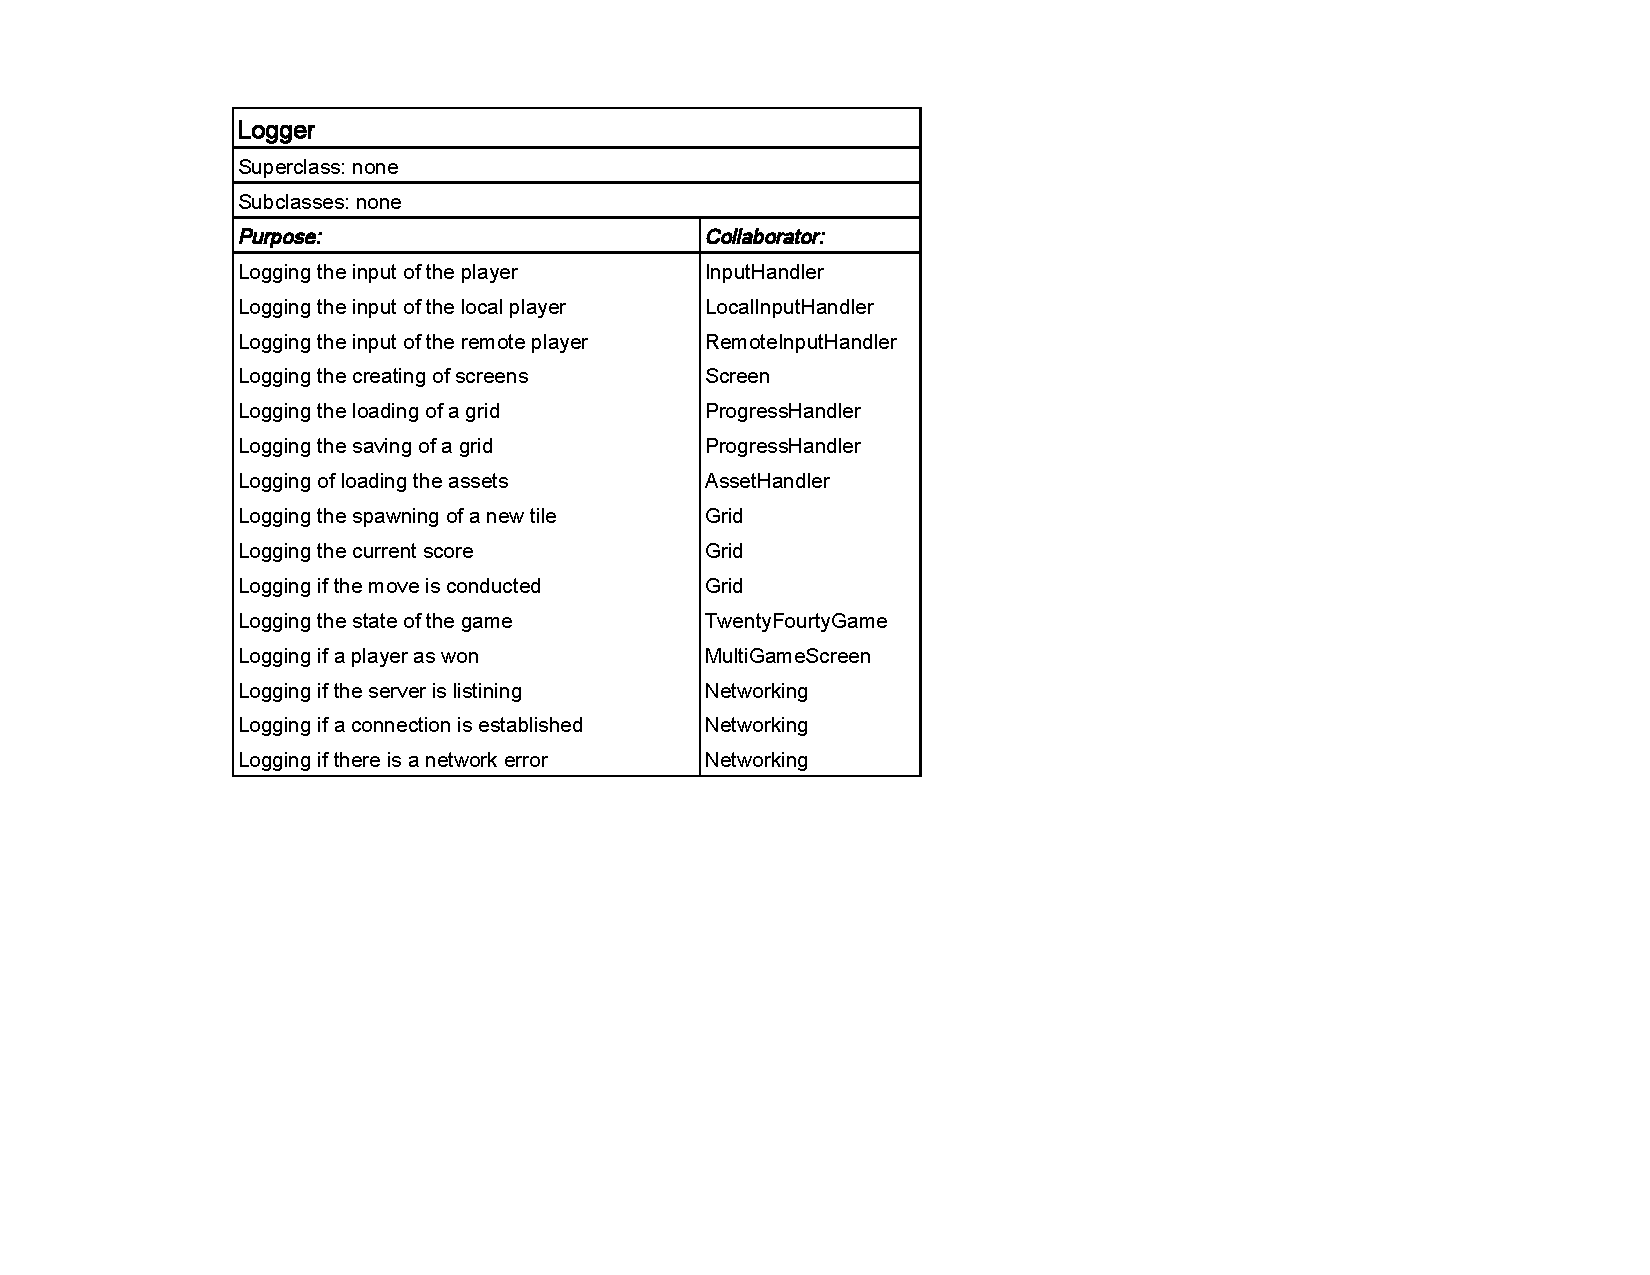
\includegraphics[trim=0 200 0 50,clip=true,scale=0.7]{sources/LoggerCRCCard}}

We have also made a small class diagram:\\

\newpage\centerline{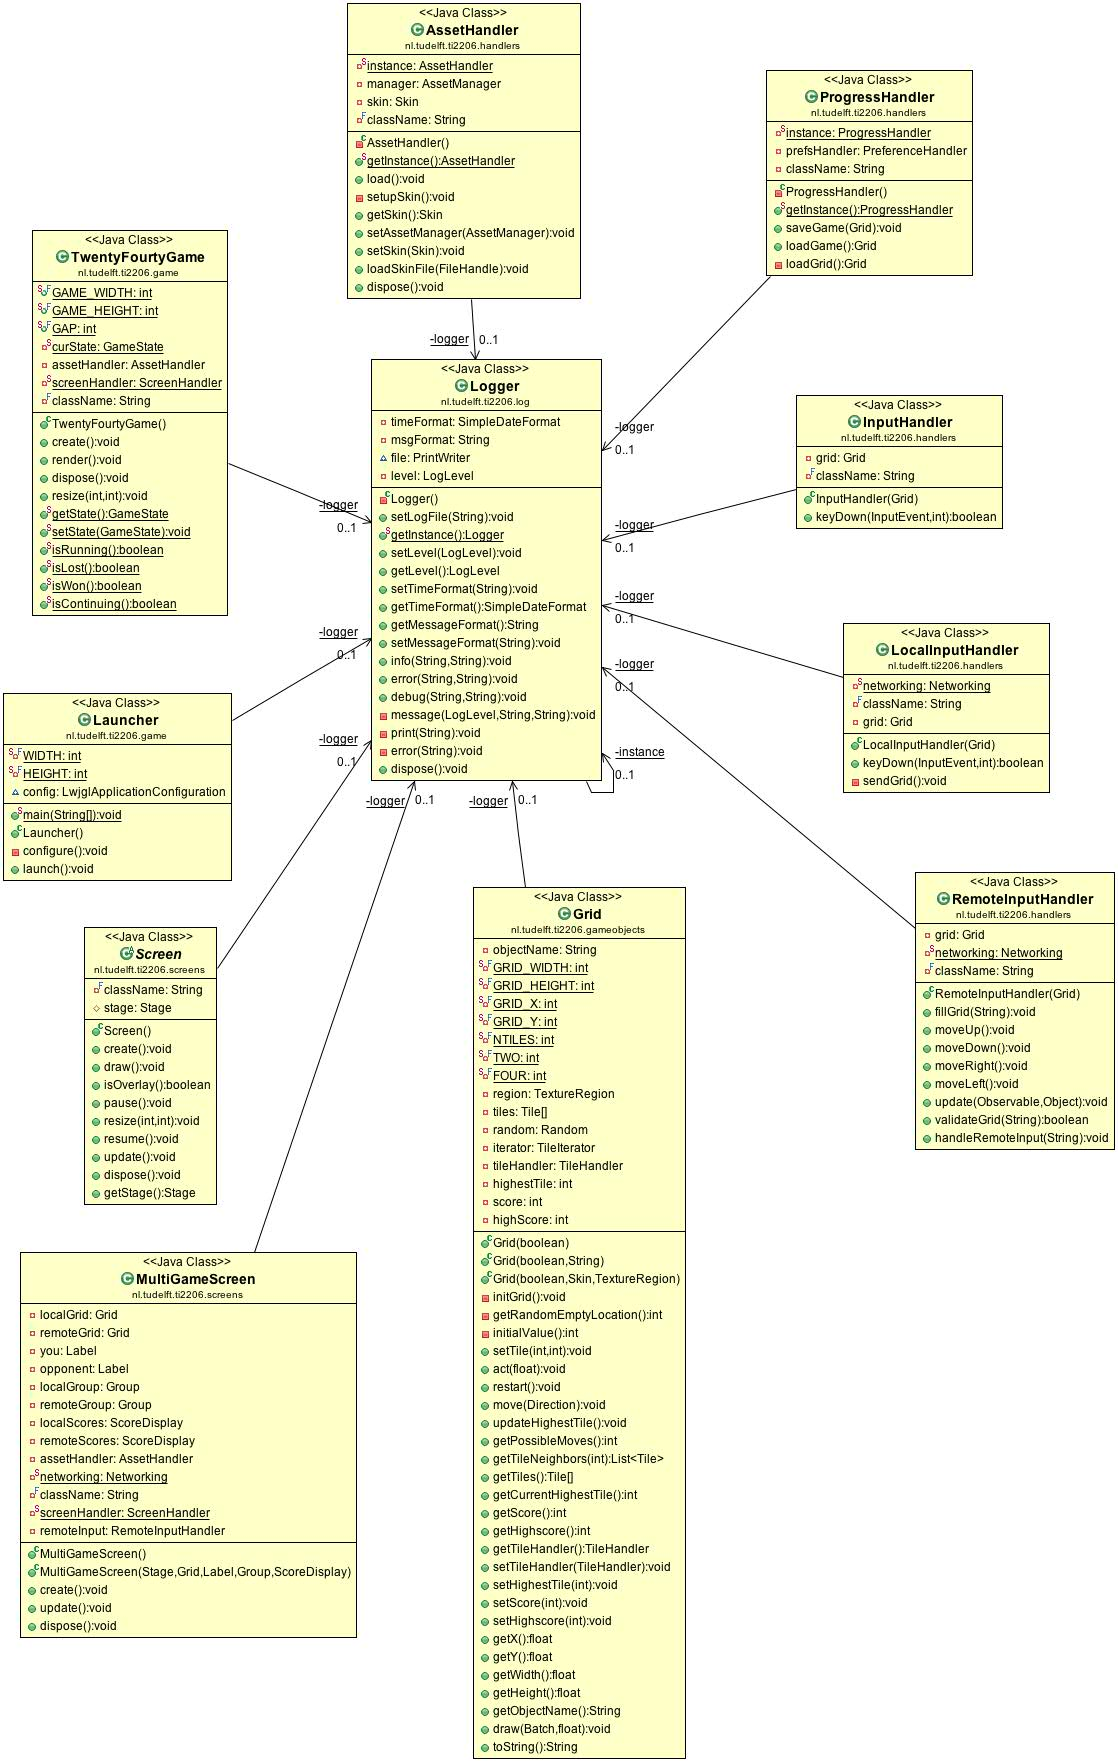
\includegraphics[trim=200 220 200 180,scale=0.47]{sources/LoggerUML}}

\newpage\section{Exercise 2 - Design patterns}
In this section we will discuss the three chosen design patterns. Per pattern,
we will provide (in natural language) a description of why and how the pattern
is implemented, together with a class- and sequence diagram.

\subsection{The Singleton design pattern}
We implemented the singleton design pattern because we noticed the large amount
of classes that only contained static methods. Nearly all of them are located in
the \texttt{handlers} package. This is logical, since handlers are supposed to carry out
one specific task, without the need of an instance of the class.\\

We noticed that the code did not really look clean with all those classnames in
front of methods. Instead, we could declare an instance variable in each class
using the static methods to access those. A requirement would be that only one
instance is allowed to exist, as it would make no sense to have multiple
instances when the class does not maintain any state. This is exactly what the
Singleton design pattern is for.

\subsubsection{The implementation}
First of all, we started refactoring the classes that were going to follow the
singleton design pattern. A static instance variable of the singleton class was
created, initializing the unique instance of the class:
\begin{verbatim}
private static Singleton instance = new Singleton();
\end{verbatim}
\newpage Since this instance is static, it already exists before a the class instance
can exist. Therefore, this approach is thread safe.\\

A private constructor was added to override the default constructor:
\begin{verbatim}
private Singleton() {}
\end{verbatim}
This constructor cannot be accessed from outside the singleton class because it
has the private modifier, so no other class can even try to create a new
instance of the singleton.\\

Then, a public static method was added for other classes to retrieve the
singleton instance:
\begin{verbatim}
public static Singleton getInstance() {
    return instance;  
}
\end{verbatim}
Since this method is static, the singleton is accessed without having to create
a new instance of the class. In classes that use the instance, we could just
add an instance variable to retrieve it once and use it throughout the code.\\

For this to actually work, the methods that used to be static were refactored
to public methods in order to be able to access them through the instance of
the singleton.

\subsubsection{The class- and sequence diagram}
\textbf{The class diagram:}\\
\centerline{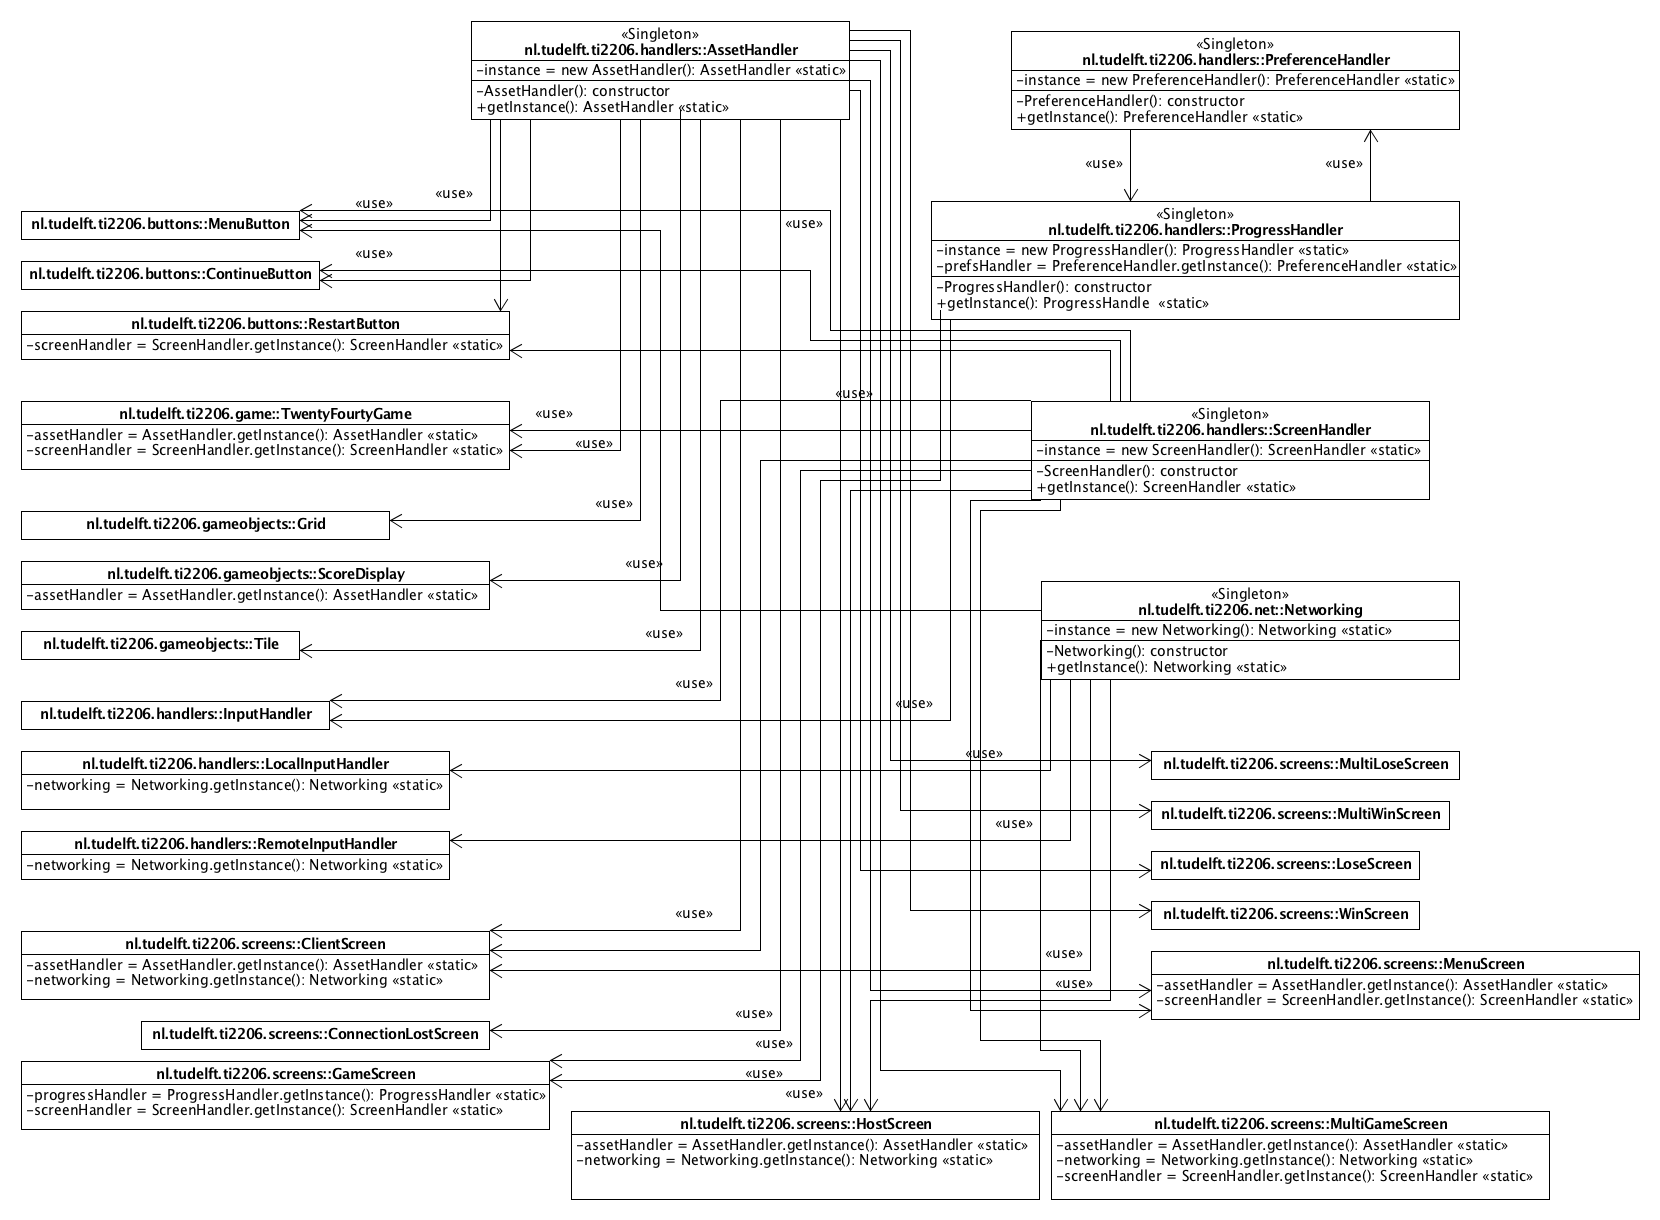
\includegraphics[scale=0.3]{sources/SingletonUML}}

\newpage\textbf{The sequence diagram:}\\
\centerline{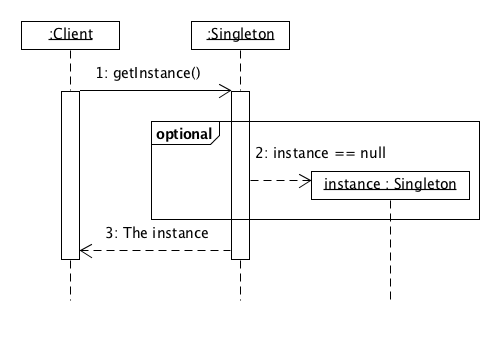
\includegraphics[scale=1.0]{sources/SingletonSequence}}

\newpage\subsection{The Iterator design pattern}
We implemented the iterator design pattern because we have to iterate over our
grid a lot. It seemed a natural choise to implement an iterator on top of this.
The prospect of having to refactor our \texttt{TileHandler} class was daunting, though,
so we never did it. This assignment, however, gave us the needed motivation to
go ahead and do it.

\subsubsection{The implementation}
A new class, the \texttt{TileIterator} class, has been created. This class implements the
\texttt{Iterator} interface that is defined in \texttt{java.util}. The classes that have to
iterate over the grid now make use of this \texttt{TileIterator}.\\

One detail we would like to point out, is that our \texttt{TileIterator} also has a reset
method. This method will move the index back to the beginning of the array, so
the iterator can be used again. This allows us to have only one instance of
\texttt{TileIterator} inside the \texttt{Grid} class instead of every method creating an iterator
when needed. This would mean that several new \texttt{TileIterator} instances would be
created sixty times per second! The same trick is used inside
\texttt{TileHandler}, although the impact here is less big.

\subsubsection{The class- and sequence diagram}
\textbf{The class diagram:}\\
\centerline{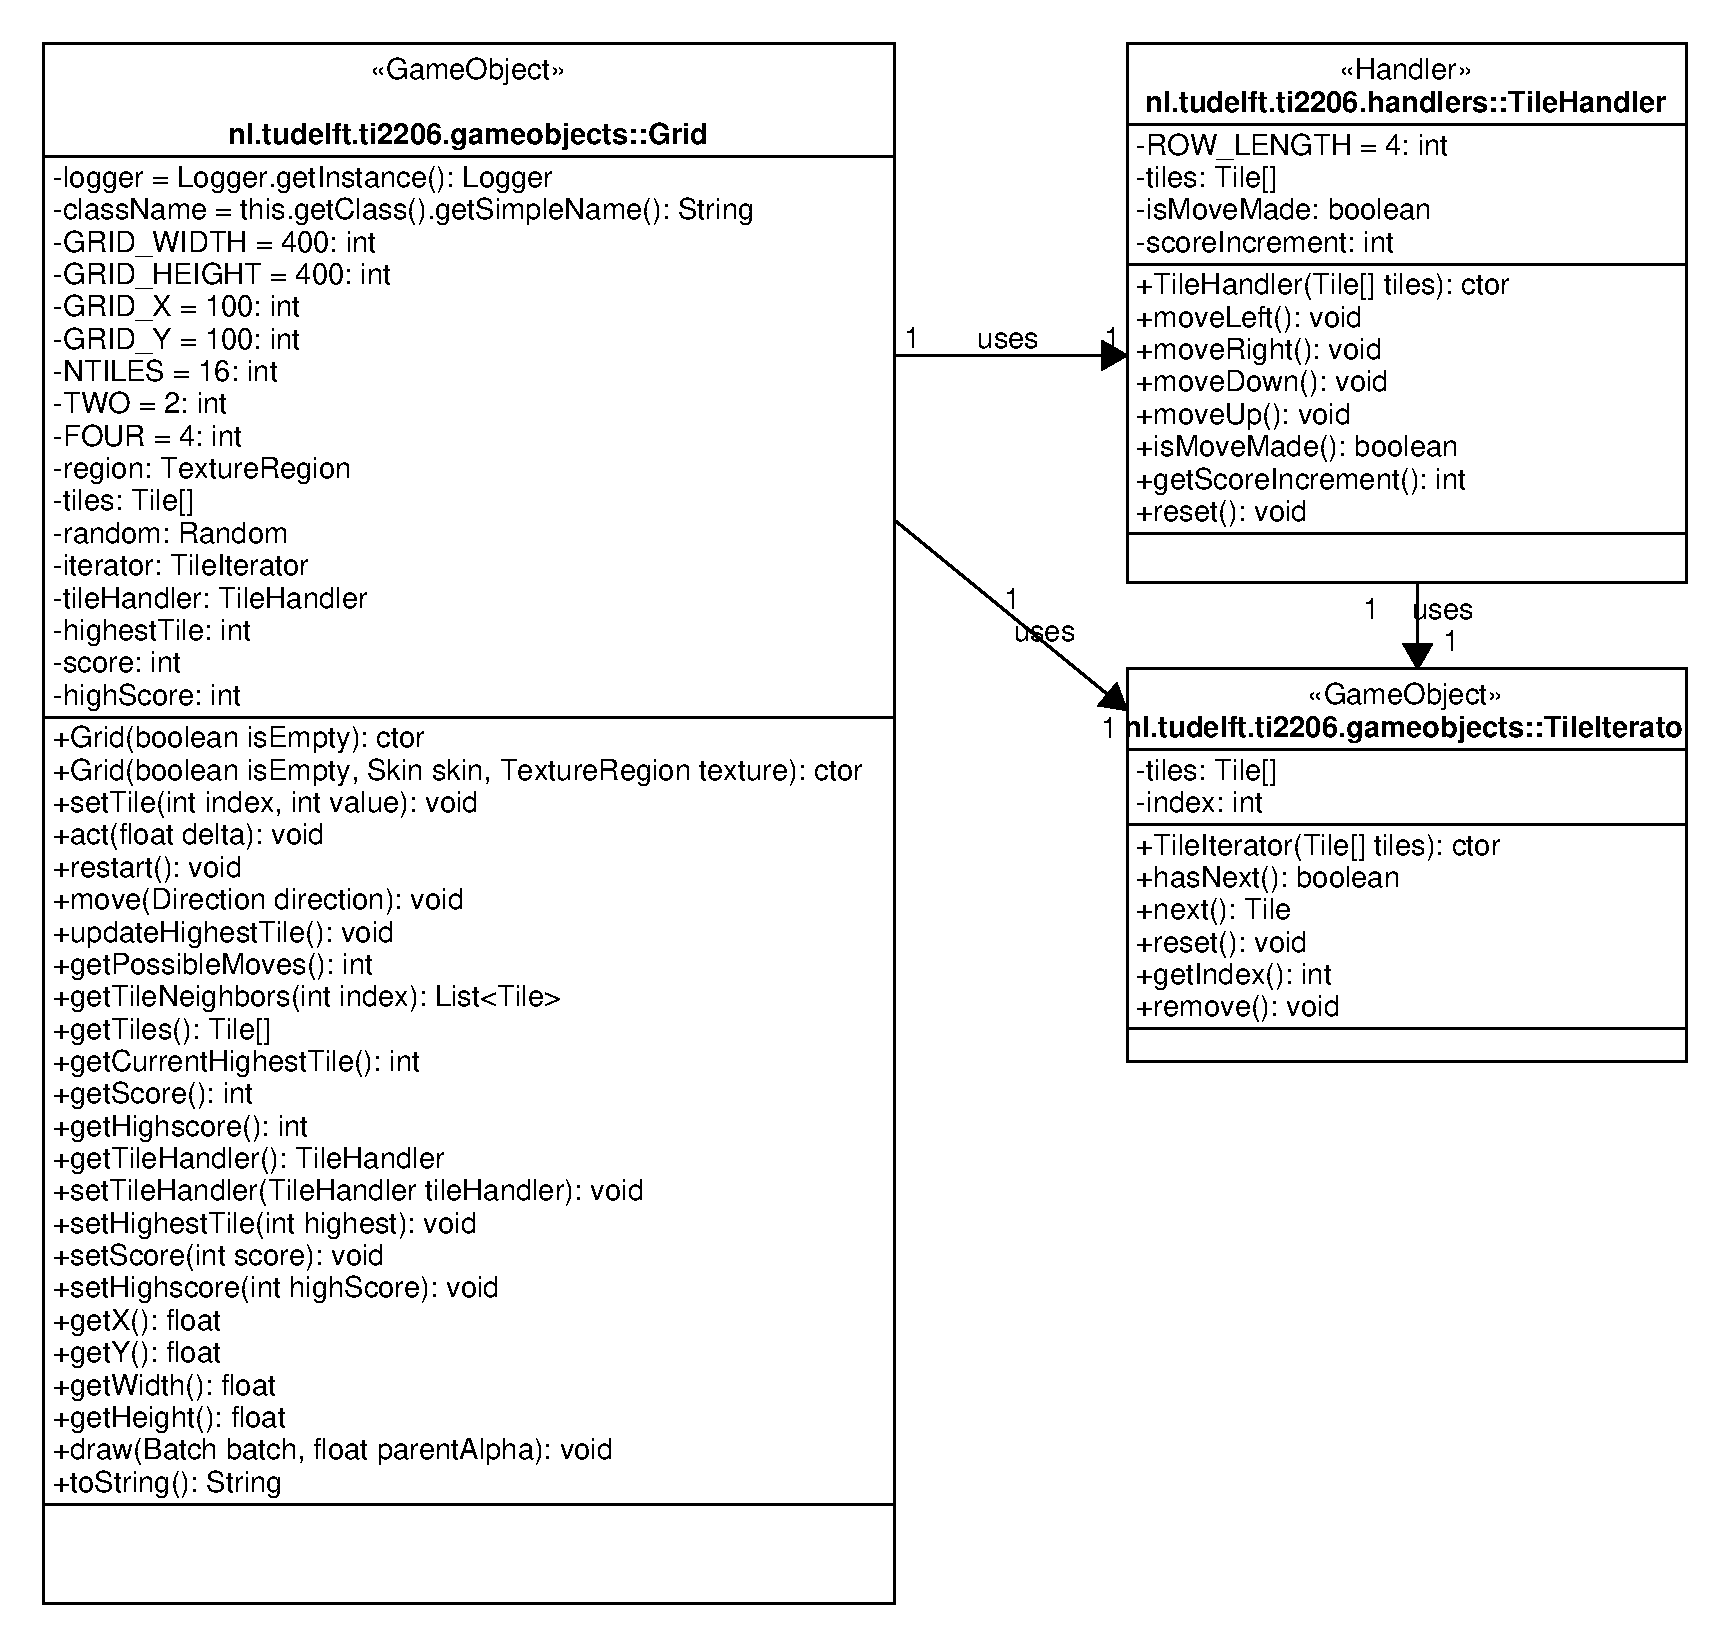
\includegraphics[scale=0.6]{sources/IteratorUML}}

\newpage\textbf{The sequence diagram:}\\
\centerline{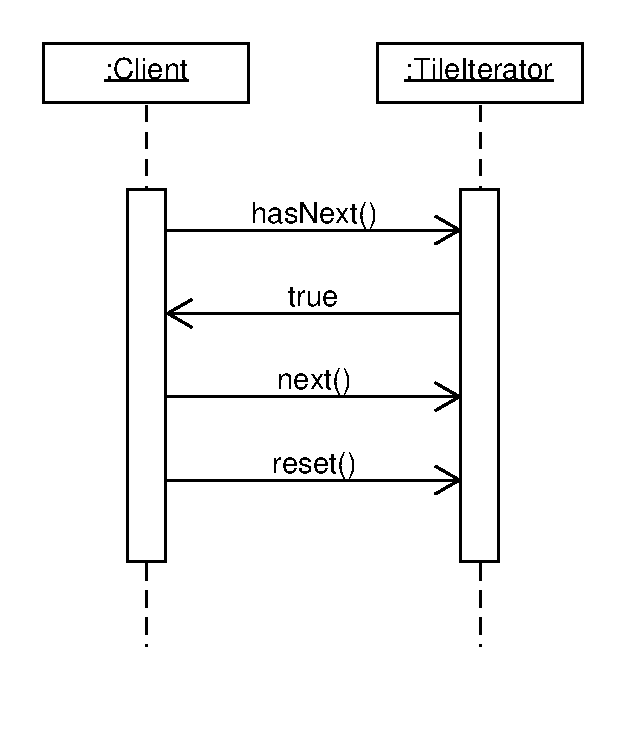
\includegraphics[scale=1.0]{sources/IteratorSequence}}

\newpage\subsection{The Observer design pattern}
The \texttt{Networking} class is required to synchronize movements and the grids.\\

In previous releases of 2048, we would give a handle to the
\texttt{RemoteInputHandler} object to the \texttt{Networking} class. This way,
however, attaches \texttt{RemoteInputHandler} entirely to \texttt{Networking}.\\

To circumvent this in our new version, the \texttt{RemoteInputHandler}
registers itself to \texttt{Networking} as an \texttt{Observer} so that the
\texttt{Observable} (the \texttt{Networking} class) can notify the
\texttt{RemoteInputHandler} whenever it needs to be updated.

\subsubsection{The implementation}
The \texttt{RemoteInputHandler} class simply gets a singleton instance of the
\texttt{Networking} class:
\begin{verbatim}
private static Networking networking = Networking.getInstance();
\end{verbatim}
Then, in its constructor, it calls the \texttt{addObserver} method on the
\texttt{Networking} object and it registers itself as a observer:
\begin{verbatim}
networking.addObserver(this);
\end{verbatim}
The \texttt{Networking} class can now send objects to the
\texttt{RemoteInputHandler} without them being fully attached to eachother.
Whenever \texttt{Networking} needs to send an object to
\texttt{RemoteInputHandler} it can simply set a flag to a changed state, using:
\begin{verbatim}
setChanged();
\end{verbatim}
and then simply notify all observers that were registered in the past:
\begin{verbatim}
notifyObservers(response);
\end{verbatim}
The benefits of this design are that \texttt{Networking} can communicate with other
objects while not being fully attached to them and newly added objects can
easily be registered to the list of observers, allowing the application to be
maintained and extended in an easier way.

\newpage\subsubsection{The class- and sequence diagram}
\textbf{The class diagram:}\\
\centerline{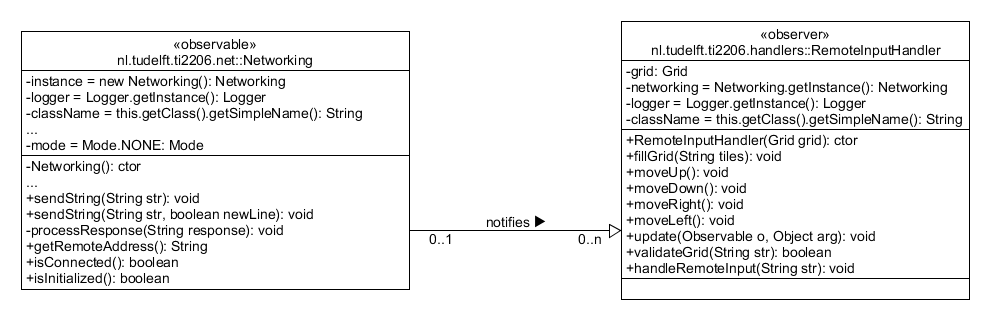
\includegraphics[scale=0.5]{sources/ObserverUML}}

\textbf{The sequence diagram:}\\
\centerline{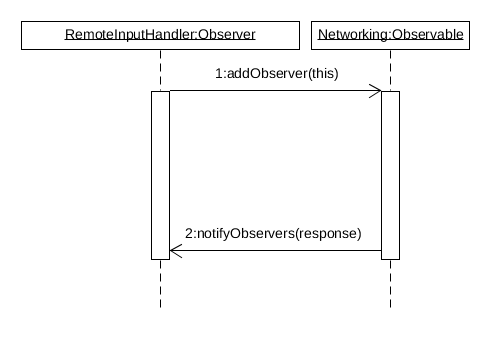
\includegraphics[scale=1.0]{sources/ObserverSequence}}

\newpage\section{Exercise 3 - One more design pattern}
We use a \texttt{Screen} hierarchy to define some of the GUI aspects that we use in the
game. The parent, \texttt{Screen}, has a draw method among others that are extended
to the child classes. These child classes would use one of two implementations
of the draw method: the implementation that was extended from the parent, or
override into a different implementation. Because of this, the classes that
override the existing method would have duplicate code.\\

By applying the Strategy design pattern to our existing hierarchy we can not
only reduce duplicate code but also prepare our program to further changes.
This has been done by encapsulating the different implementations in a family
of algorithms. Every class can now add one of the objects to use an implementation
dynamically (even in runtime), instead of implementing it by themselves. As
the program grows and a new set of screens with a different implementation
of the draw method is added, we can simply add a new class to the family
in which define the implementation, without forcing any changes in the existing
classes.

\subsubsection{The implementation}
The pattern has been implemented by moving the existing implementations of the
draw method into separated classes that implement the \texttt{DrawBehavior} interface.
This interface contains a draw method that the implementing classes override
with their own implementation. By adding a local variable to the
\texttt{Screen} class and a method to assign a new \texttt{DrawBehavior} object to it, a
\texttt{DrawBehavior} object can be assigned to every screen object to determine its
draw implementation.

\newpage\subsubsection{The class- and sequence diagram}
\textbf{The class diagram:}\\
\centerline{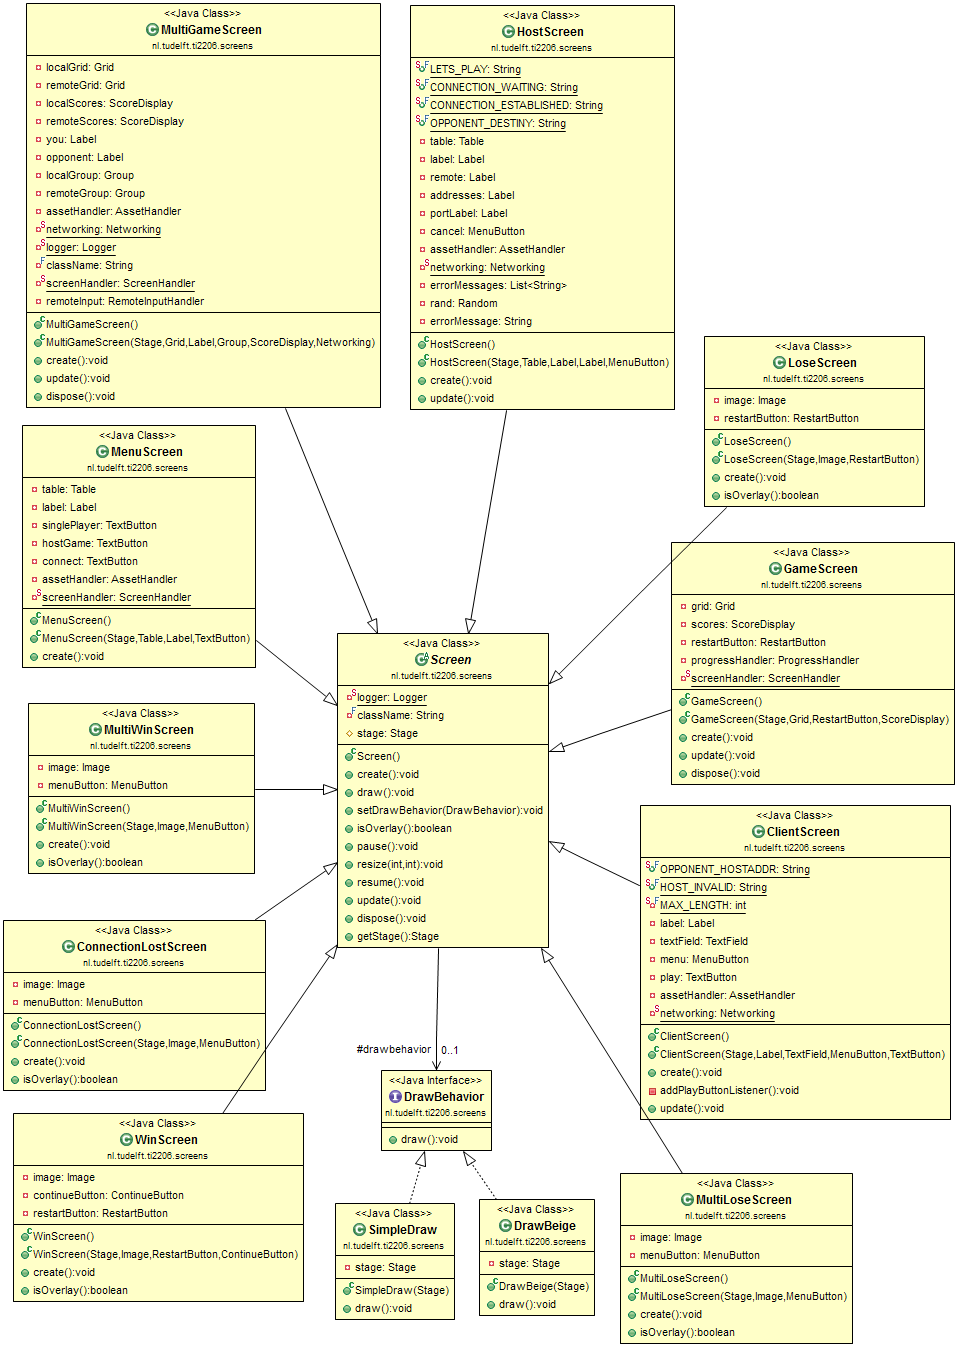
\includegraphics[scale=0.40]{sources/StrategyUML}}

\newpage\textbf{The sequence diagram:}\\
\centerline{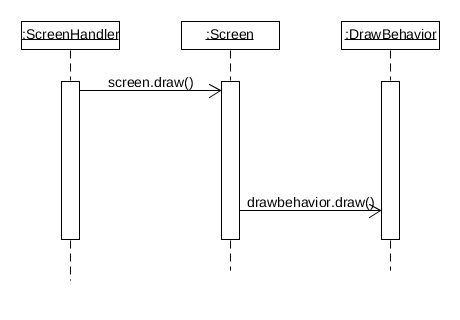
\includegraphics[scale=1.0]{sources/StrategySequence}}

\end{document}
